\subsection{Mesa de posicionamento}

% SLIDE DE MESA DE POSICIONAMENTO
\begin{frame}
\frametitle{Mesa de posicionamento}

Podem ser classificadas em dois tipos com relação a sua transmissão: as mesas acionadas por fusos e por correias sincronizadas.

\begin{columns}
    \column{0.5\textwidth}
        \begin{figure}
        \centering
        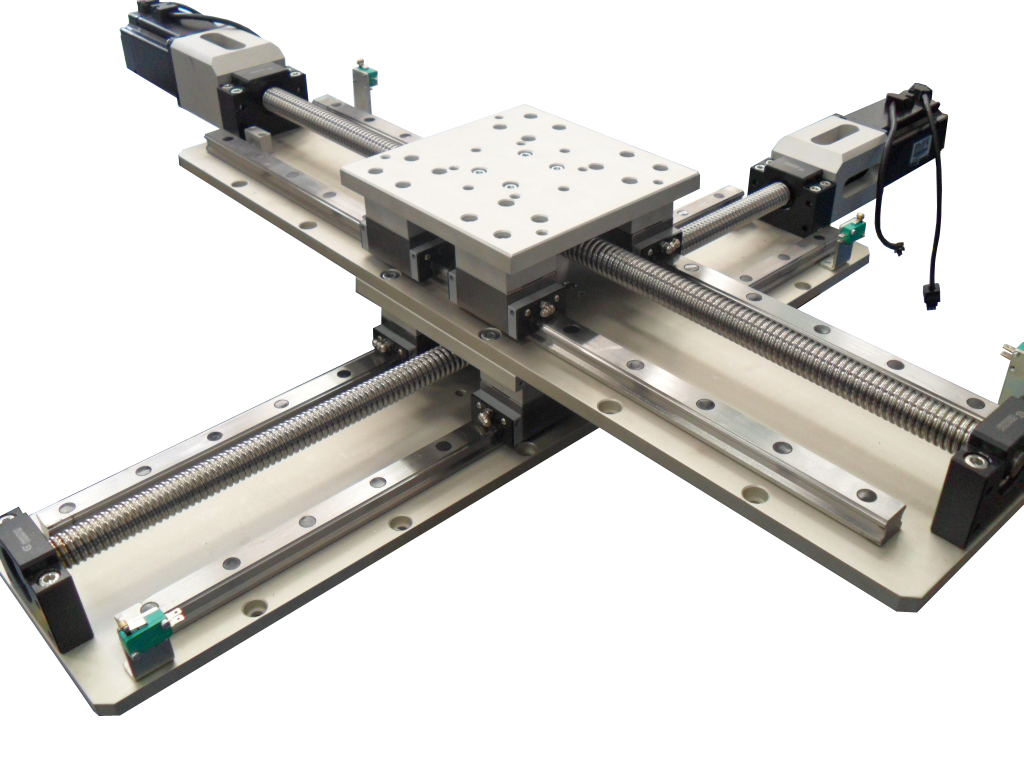
\includegraphics[scale = 0.12]{figuras/mfuso}
        \end{figure}
    \column{0.5\textwidth}
        \begin{figure}
        \centering
        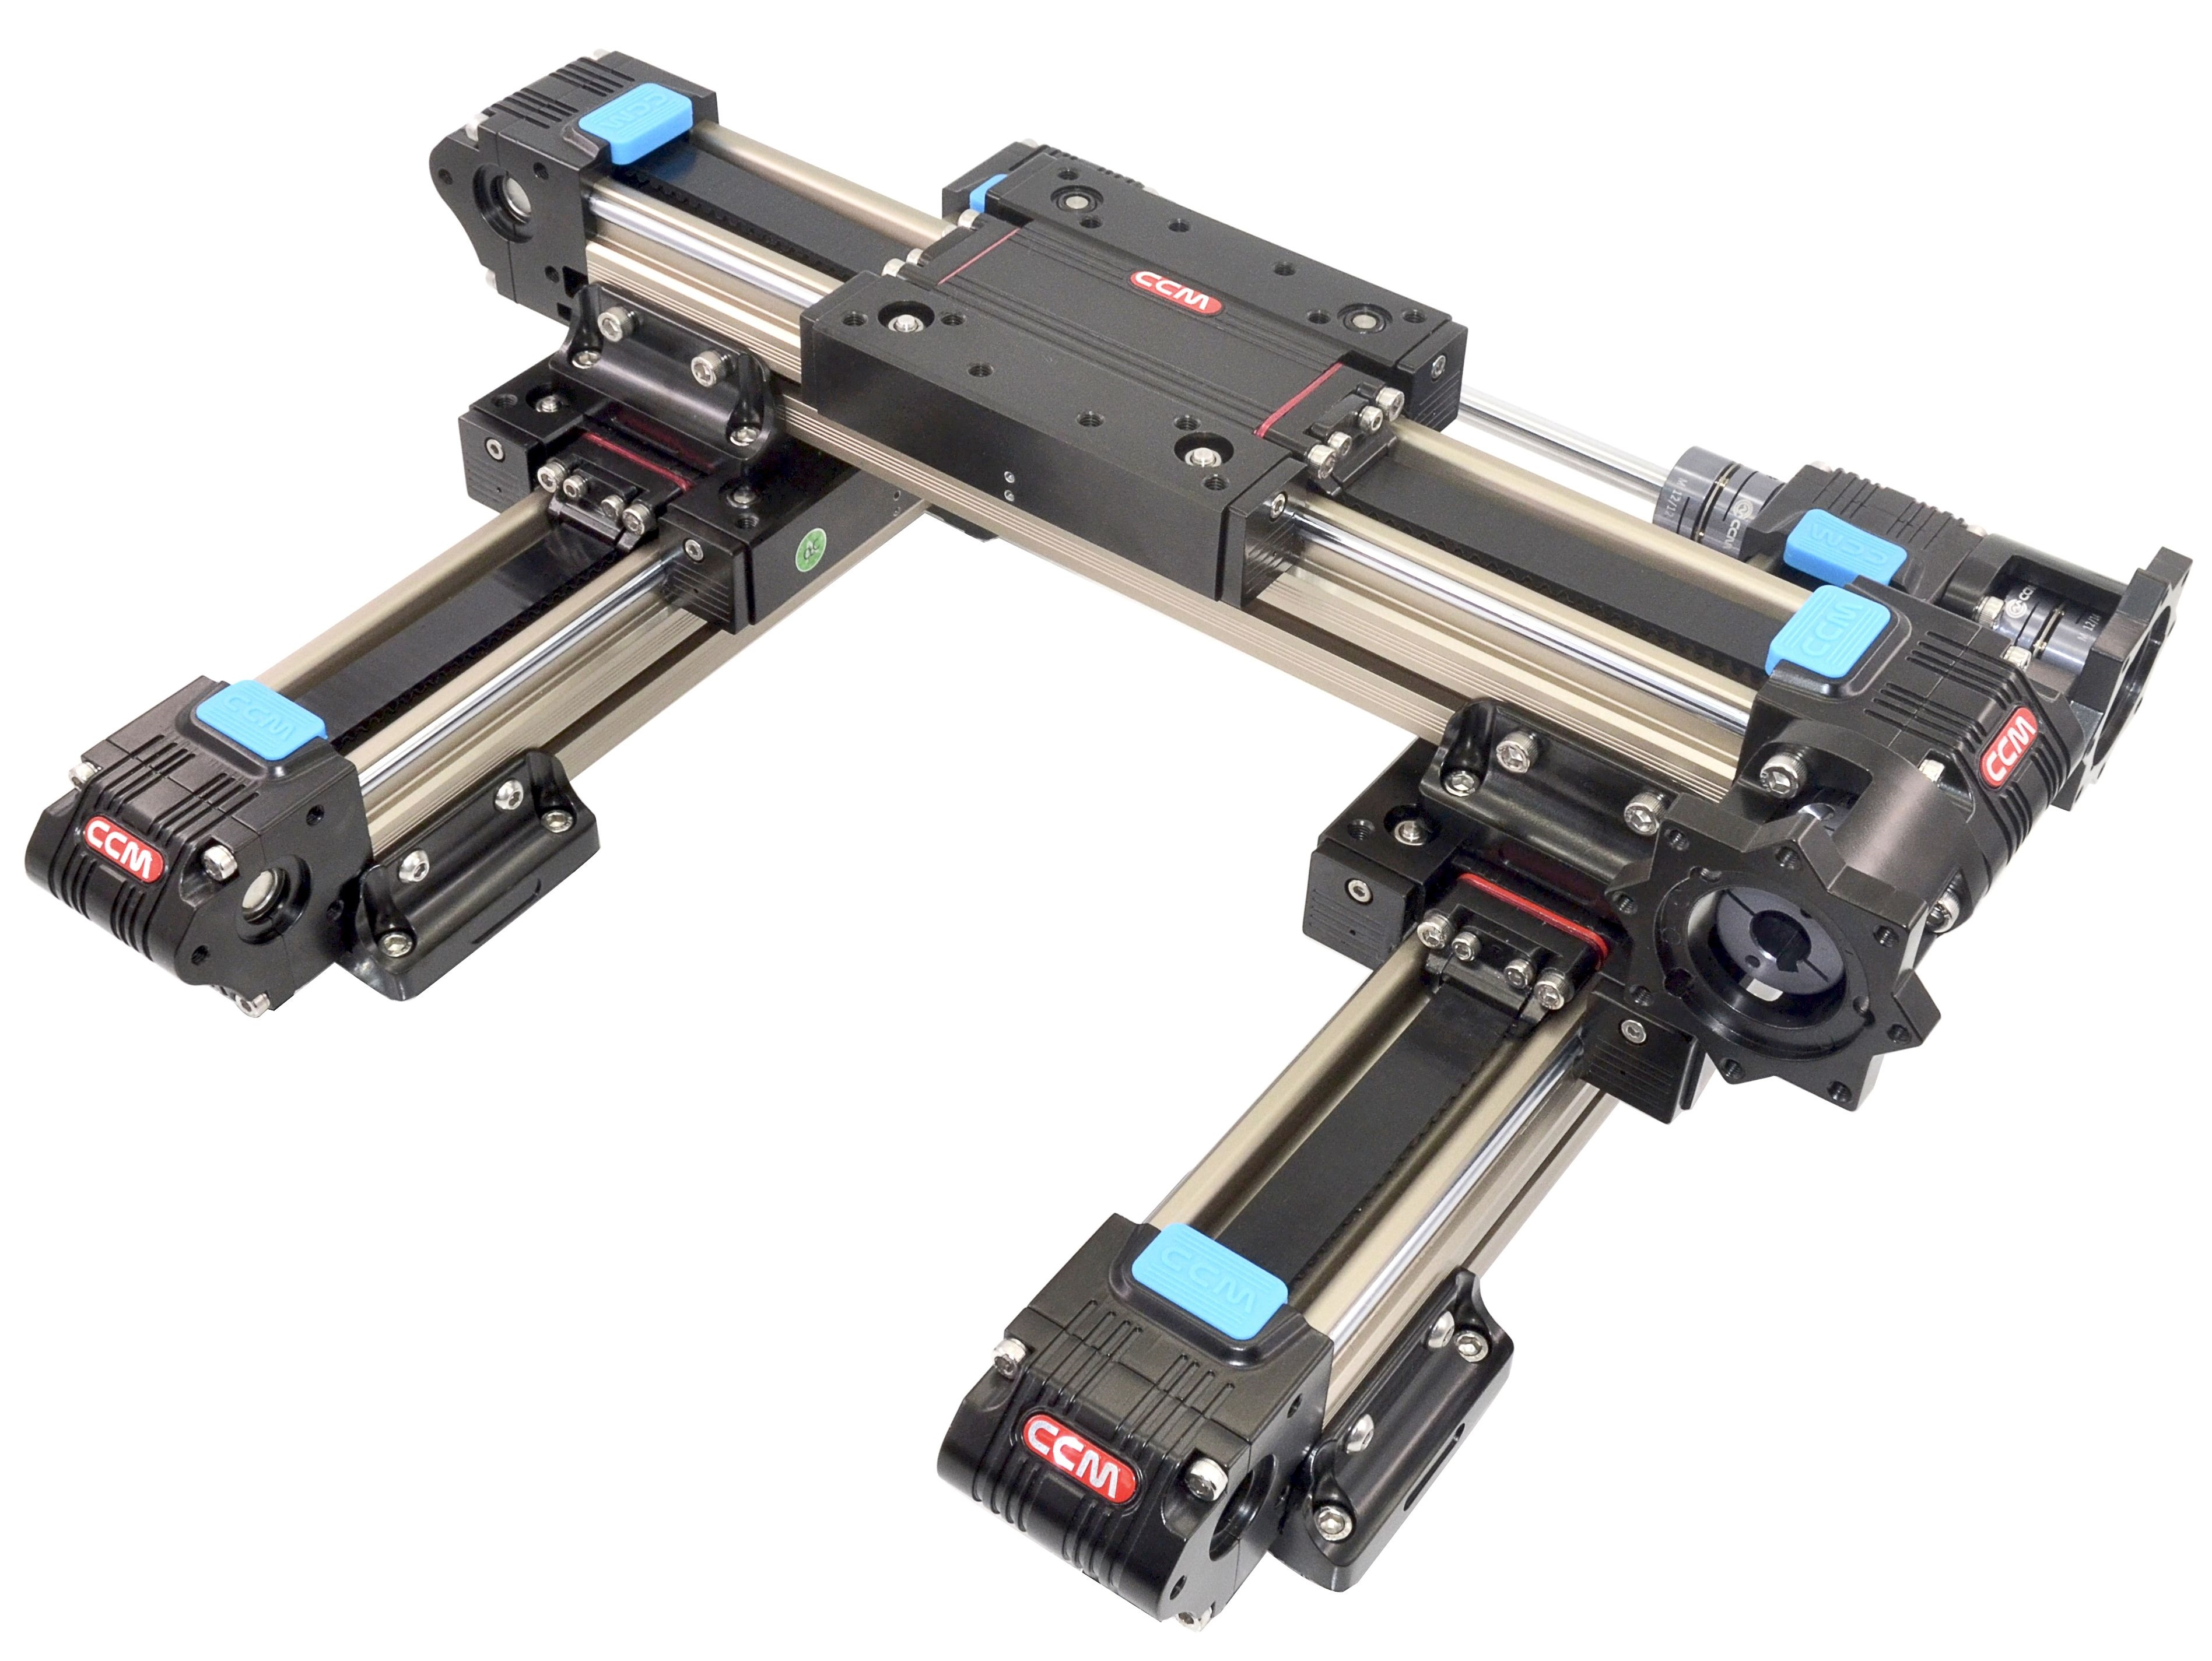
\includegraphics[scale = 0.03]{figuras/mcorreia}
        \end{figure}
\end{columns}

\end{frame}
    
% SLIDE DE MESA DE POSICIONAMENTO
\begin{frame}
\frametitle{Mesa de posicionamento}

Outro componente importante é o acionador, que pode ser um motor de passo. 

Os motores de passo são máquinas utilizadas em aplicações de um alto grau de precisão no movimento em passos fixos, referentes a uma fração de ângulo. 

\begin{figure}
\centering
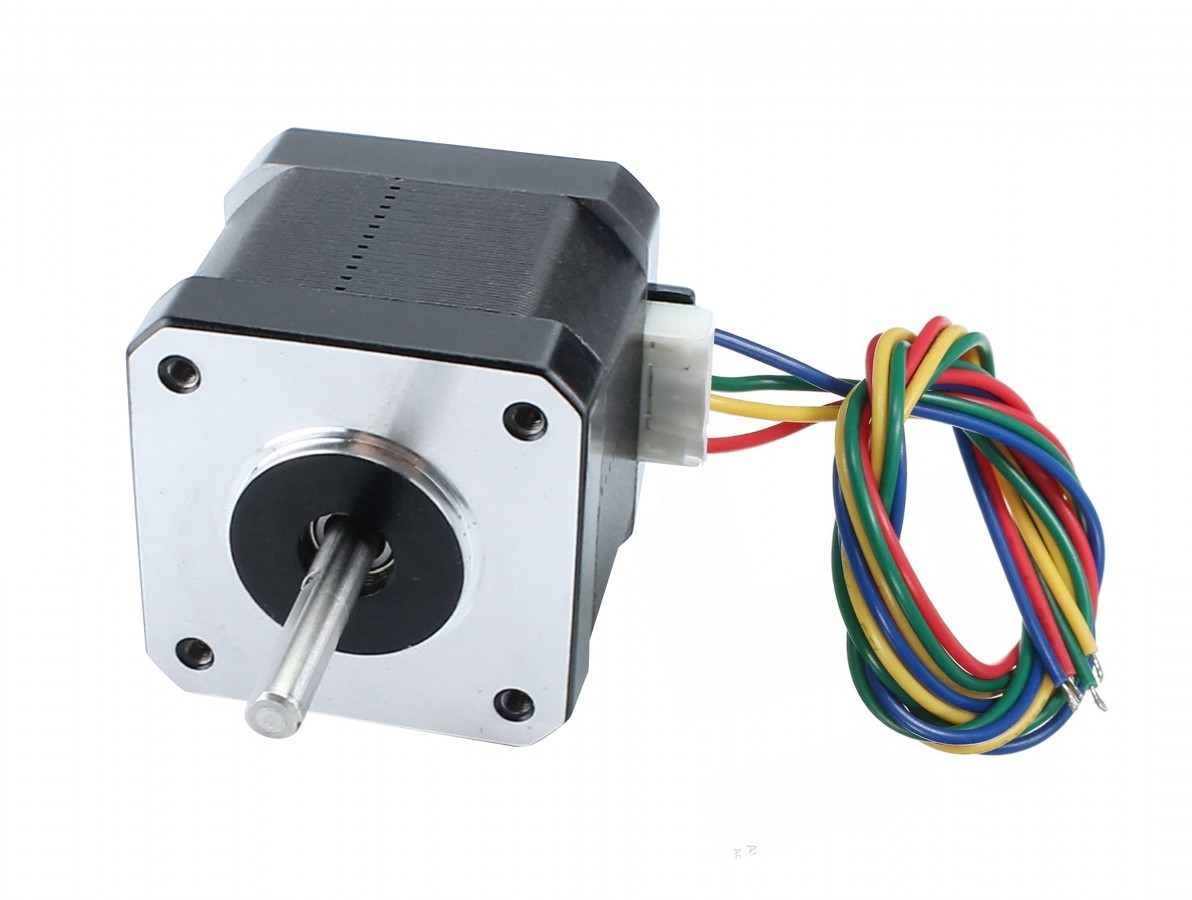
\includegraphics[scale = 0.07]{figuras/motordepassoex}
\end{figure}
\end{frame}
